\section{Tight-binding model Dirac}

We start with a nearest-neighbor single-orbital tight-binding Hamiltonian

\begin{equation}
  \ham = - \sum_{jl\alpha,j'l'\beta} h \cc_{jl\alpha} c_{j'l'\beta} + h.c.
\end{equation}
The incident laser beam in vector potential forms looks like

\begin{equation} \label{eq:AvecDirac}
  \vec{A}(\vec{r},t) = \dfrac{E}{\omega} \langle -\sin \omega t, \dfrac{1}{2} \sin(Kx) \cos 2\omega t \rangle.
\end{equation}
Using the following approximation for smoothly varying vector potential fields

\begin{equation}
  \int_{\vec{r}_{j,l}^{\alpha}} ^{\vec{r}_{j',l'}^{\beta}} \vec{A}(\vec{r},t) \cdot d\vec{l} \approx \vec{A} \left( \dfrac{ \vec{r}_{j',l'}^{\beta} + \vec{r}_{j,l}^{\alpha} }{2}, t \right) \cdot \left( \vec{r}_{j',l'}^{\beta} - \vec{r}_{j,l}^{\alpha} \right)
\end{equation}


where

\begin{align}
  \vec{a}_1 &= \sqrt{3}a\hat{x} \\
  \vec{a}_2 &= 3a\hat{y} \\
  \vec{r}_{jl}^{A_1} &= j\vec{a}_1 + l\vec{a}_2 \\
  \vec{r}_{jl}^{B_1} &= (j+\tfrac{1}{2})\vec{a}_1 + (l+\tfrac{1}{6})\vec{a}_2 \\
  \vec{r}_{jl}^{A_2} &= (j+\tfrac{1}{2})\vec{a}_1 + (l+\tfrac{1}{2})\vec{a}_2 \\
  \vec{r}_{jl}^{B_2} &= (j+1)\vec{a}_1 + (l+\tfrac{2}{3})\vec{a}_2.
\end{align}

\begin{figure}[h]
  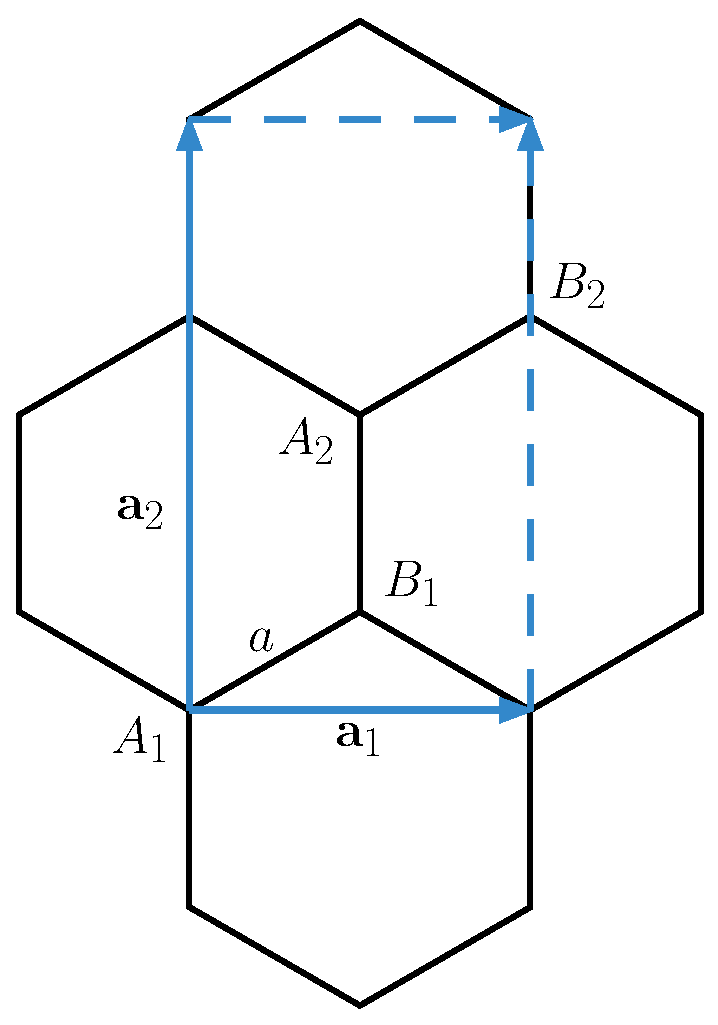
\includegraphics[width=0.30\textwidth]{./dirac-floquet-unit-cell.pdf}
\caption{Unit cell for dirac system with gauge potential with tranlation symmetry in the $y-axis$ described by Eq.~\eqref{eq:AvecDirac}.}
  \label{fig:dirac-floquet-unit-cell}
\end{figure}
Applying a Peierls substitution the Hamiltonian becomes

\begin{equation}
\begin{split}
  \ham (t) = -\sum_{jl} \ &h_{jlA_1}^{jlB_1}(t) \cc_{jlA_1} c_{jlB_1} + h_{jlB_1}^{jlA_2}(t) \cc_{jlB_1} c_{jlA_2} + h_{jlA_2}^{jlB_2}(t) \cc_{jlA_2} c_{jlB_2} \\
      + &h_{jlB_1}^{j+1,lA_1}(t) \cc_{jlB_1} c_{j+1,lA_1} + h_{jlB_2}^{j+1,l,A_2} \cc_{jlB_2} c_{j+1,lA_2}(t) \\
      + &h_{jlB_2}^{j+1,l+1,A_1}(t) \cc_{jlB_2} c_{j+1,l+1,A_1} + h.c.
\end{split}
\end{equation}
where in general

\begin{equation}
  h_{jl\alpha}^{j'l'\beta} (t) \approx h \exp \left[ i \phi_0 \left(-\dfrac{x_{j'l'}^{\beta} - x_{jl}^{\alpha}}{a} \sin\omega t + \dfrac{y_{j'l'}^{\beta} - y_{jl}^{\alpha}}{2a} \cos\left(K \dfrac{x_{j'l'}^{\beta} + x_{jl}^{\alpha}}{2}\right) \cos 2\omega t \right) \right],
\end{equation}
where $\phi_{0} = eE/(\hbar \omega)$.
More explicitly for each term

\begin{align}
  h_{jlA_1}^{jlB_1}(t) &\approx h \exp \left[ i\phi_0 \left(-\dfrac{\sqrt{3}}{2} \sin\omega t + \dfrac{1}{4} \sin(\sqrt{3}Ka(j+\tfrac{1}{4})) \cos 2\omega t \right) \right] \\
  h_{jlB_1}^{jlA_2}(t) &\approx h \exp \left[ i\phi_0 \left(\dfrac{1}{2} \sin(\sqrt{3}Ka(j+\tfrac{1}{2})) \cos 2\omega t \right) \right] \\
  h_{jlA_2}^{jlB_2}(t) &\approx h \exp \left[ i\phi_0 \left(-\dfrac{\sqrt{3}}{2} \sin\omega t + \dfrac{1}{4} \sin(\sqrt{3}Ka(j+\tfrac{3}{4})) \cos 2\omega t \right) \right]
\end{align}
\begin{align}
  h_{jlB_1}^{j+1,lA_1}(t) &\approx h \exp \left[ i\phi_0 \left(-\dfrac{\sqrt{3}}{2} \sin\omega t - \dfrac{1}{4} \sin(\sqrt{3}Ka(j+\tfrac{3}{4})) \cos 2\omega t \right) \right] \\
  h_{jlB_2}^{j+1,lA_2}(t) &\approx h \exp \left[ i\phi_0 \left(-\dfrac{\sqrt{3}}{2}\sin\omega t -\dfrac{1}{4} \sin(\sqrt{3}Ka(j+\tfrac{5}{4})) \cos 2\omega t \right) \right] \\
  h_{jlB_2}^{j+1,l+1,A_1}(t) &\approx h \exp \left[ i\phi_0 \left(\dfrac{1}{2} \sin(\sqrt{3}Ka(j+1)) \cos 2\omega t \right) \right]
\end{align}

The incident laser beam allows for translation symmetry along the y-axis, so we can reduce the dimension of the Hamiltonian with the following Fourier transform

\begin{equation}
  \cc_{jl\alpha} = \dfrac{1}{N_y} \sum_k \cc_{jk\alpha} e^{ik\hat{y}\cdot\vec{R_l}} = \dfrac{1}{N_y} \sum_k \cc_{jk\alpha} e^{ik(3la)}
\end{equation}
The Hamiltonian then becomes

\begin{equation}
\begin{split}
  \ham (t) = -\sum_{jk} \ &h_{jlA_1}^{jlB_1}(t) \cc_{jkA_1} c_{jkB_1} + h_{jlB_1}^{jlA_2}(t) \cc_{jkB_1} c_{jkA_2} + h_{jlA_2}^{jlB_2}(t) \cc_{jkA_2} c_{jkB_2} \\
      + &h_{jlB_1}^{j+1,lA_1}(t) \cc_{jkB_1} c_{j+1,kA_1} + h_{jlB_2}^{j+1,l,A_2} \cc_{jkB_2} c_{j+1,kA_2}(t) \\
      + &h_{jlB_2}^{j+1,l+1,A_1}(t) e^{-i3ka} \cc_{jkB_2} c_{j+1,kA_1} + h.c.
\end{split}
\end{equation}

Making use of Floquet theory we can make the Hamiltonian time-independent with the following time domain Fourier transform

\begin{equation}
  H_{ab,n,k} = \dfrac{1}{2\pi} \int_0^{2\pi} \ham_{ab}(k,t) e^{-in\tau} d\tau
\end{equation}
where $a,b$ represent the matrix indes of the previous Hamiltonian and $n$ is the $n$-th order mode of light.
Each term has the general following form

\begin{equation}
  H_{ab,n,k} = \dfrac{1}{2\pi} \int_0^{2\pi} e^{i Z_1 \sin\tau + i Z_2 \cos2\tau - in\tau} d\tau
\end{equation}
which looks a lot like the Hansen-Bessel integral function.
However, because of the linear combination of $\sin\tau$ and $\cos 2\tau$, there is no elementary solution to the integral as currently defined.
We thus solve the integral numerically for each given $n$.
After the time domain Fourier transform the Hamiltonian can be reduced to the following matrix form
\begin{equation}
  H_n = -\sum_{jk} \left[ \Psi_{jk}^{\dagger} H_{jj} \Psi_{jk} + \Psi_{jk}^{\dagger} H_{j,j+1,k}' \Psi_{j+1,k} + h.c. \right]
\end{equation}

\[
  H_{j,j} =
  \begin{bmatrix}
    0 & 0 & 0 & 0 \\
    h^{jlA_1}_{jlB_1} & 0 & 0 & 0 \\
    0 & h^{jlB_1}_{jlA_2} & 0 & 0 \\
    0 & 0 & h^{jlA_2}_{jlB_2} & 0 \\
  \end{bmatrix}
\]
and
\[
  H'_{j,j+,k} =
  \begin{bmatrix}
    0 & h^{j+1,lA_1}_{jlB_1} & 0 & h^{j+1,l+1,A_1}_{jlB_2} e^{i\vec{k}\cdot\vec{a}_2} \\
    0 & 0 & 0 & 0 \\
    0 & 0 & 0 & h^{j+1,lA_2}_{jlB_2} \\
    0 & 0 & 0 & 0
  \end{bmatrix},
\]
with $\vec{k} = k\hat{y}$ and $\Psi_{jk} = [c_{jkA_1}, c_{jkB_1}, c_{jkA_2}, c_{jkB_2}]^T$.

The quasienergy energy matrix has elements $Q_{m,m+n} = H_n - m\hbar\omega\delta_{n0}$.
We choose a cutoff for mode $m$, $|m|\leq m_c$, where $m_c$ is a positive integer.
This cuts the matrix down to have $N_m = 2m_c+1$ diagonal blocks, where each block is of size a $N_S = 2r_c +1$ square matrix, $H_n$, and $r_c$ is the cutoff radius of unit cells.
The matrix can be solved using an eigenvalue solver, producing $N_m N_S$ eigenenergies and eigenvectors for a given electric field strength $E$.
It is difficult to glean any information from looking at all the energies but one can do a projection to the $m=0$ mode to highlight which energies belong to it.
This is still not all that imformative because when using a finite system we discretize the brillouin zone uniformly and it does not necessarily mean we are picking energy values close to the folded in Dirac point, since the unperturbed brillouin zone gets folded into the perturbed smaller brillouin zone.
